\tikzstyle{list} = [rectangle, draw, text width = 3em, text centered, rounded corners]
\tikzstyle{line} = [draw, -latex']
\tikzstyle{arrow} = [thick,->,>=stealth]

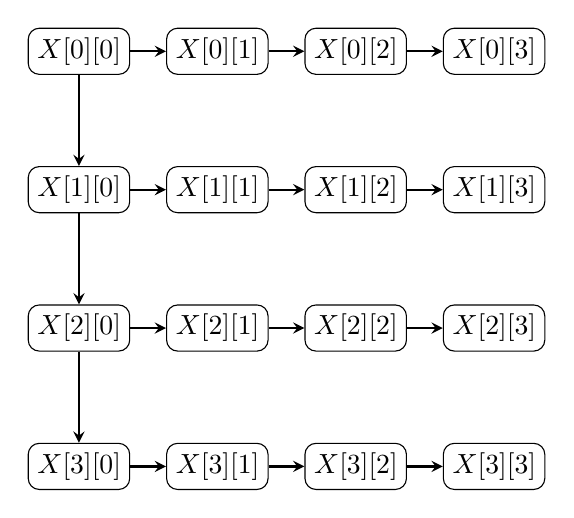
\begin{tikzpicture}
    [node distance = 5em, auto]
  \node[list] (A) {$X[0][0]$};
  \node[list, right of=A] (B) {$X[0][1]$};
  \node[list, right of=B] (C) {$X[0][2]$};
  \node[list, right of=C] (D) {$X[0][3]$};
  \node[list, below of=A] (E) {$X[1][0]$};
  \node[list, below of=B] (F) {$X[1][1]$};
  \node[list, below of=C] (G) {$X[1][2]$};
  \node[list, below of=D] (H) {$X[1][3]$};
  \node[list, below of=E] (I) {$X[2][0]$};
  \node[list, below of=F] (J) {$X[2][1]$};
  \node[list, below of=G] (K) {$X[2][2]$};
  \node[list, below of=H] (L) {$X[2][3]$};
  \node[list, below of=I] (M) {$X[3][0]$};
  \node[list, below of=J] (N) {$X[3][1]$};
  \node[list, below of=K] (O) {$X[3][2]$};
  \node[list, below of=L] (P) {$X[3][3]$};
  \draw [arrow] (A) -- (B);
  \draw [arrow] (B) -- (C);
  \draw [arrow] (C) -- (D);
  \draw [arrow] (A) -- (E);
  \draw [arrow] (E) -- (F);
  \draw [arrow] (F) -- (G);
  \draw [arrow] (G) -- (H);
  \draw [arrow] (E) -- (I);
  \draw [arrow] (I) -- (J);
  \draw [arrow] (J) -- (K);
  \draw [arrow] (K) -- (L);
  \draw [arrow] (I) -- (M);
  \draw [arrow] (M) -- (N);
  \draw [arrow] (N) -- (O);
  \draw [arrow] (O) -- (P);
\end{tikzpicture}